\documentclass[conference]{IEEEtran}
\IEEEoverridecommandlockouts
% The preceding line is only needed to identify funding in the first footnote. If that is unneeded, please comment it out.
\usepackage{cite}
\usepackage{amsmath,amssymb,amsfonts}
\usepackage{algorithmic}
\usepackage{graphicx}
\usepackage{textcomp}
\usepackage{xcolor}
\usepackage{float}
\def\BibTeX{{\rm B\kern-.05em{\sc i\kern-.025em b}\kern-.08em
    T\kern-.1667em\lower.7ex\hbox{E}\kern-.125emX}}
\begin{document}

\title{Conference Paper Title*\\
{\footnotesize \textsuperscript{*}Note: Sub-titles are not captured in Xplore and
should not be used}
\thanks{Identify applicable funding agency here. If none, delete this.}
}

\author{\IEEEauthorblockN{1\textsuperscript{st} Amardeep Singh Dhillon}
\IEEEauthorblockA{\textit{Department of Mathematics and Computing} \\
\textit{Mount Royal University}\\
Calgary, Canada \\
adhil365@mtroyal.ca , ORCID:0009-0009-7729-3060}
}

\maketitle

\begin{abstract}
This paper presents a sentiment analysis project using the Sentiment140 dataset, consisting of 1.6 million labeled Twitter tweets. 
The objective is to classify tweets as either positive or negative based on their sentiment, providing insights into public opinion on social media.
 The data was preprocessed by removing noisy elements such as URLs and user mentions, expanding abbreviations, and applying lemmatization for text normalization. 
 Various machine learning models, including Logistic Regression and Support Vector Machines (SVM), were employed for sentiment classification. Model performance 
 was evaluated using accuracy, precision, recall, and F1-score. Our results showed that the SVM model outperformed others, providing the highest accuracy. This work 
 contributes to the field of sentiment analysis, with applications in business intelligence and social media trend analysis.
\end{abstract}


\begin{IEEEkeywords}
Sentiment Analysis, Machine Learning, SVM, Logistic Regression, Sentiment140 Dataset, Text Preprocessing, Twitter Data
\end{IEEEkeywords}

\section{Introduction}
Sentiment analysis is the task of determining the sentiment expressed in a piece of text, 
which can be classified as positive, negative, or neutral. With the proliferation of social media platforms such as Twitter, 
analyzing public opinion has become more accessible. Sentiment analysis of Twitter data can be particularly valuable for businesses, 
researchers, and policymakers who want to understand the views and emotions of the public. This project aims to classify tweets as either p
ositive or negative based on their sentiment using the Sentiment140 dataset. This dataset provides a large-scale, labeled collection of tweets, 
making it a popular benchmark for sentiment analysis tasks. However, working with raw Twitter data presents challenges due to its informal nature, 
the presence of slang, and irrelevant content like URLs and user mentions.

\section{Related Work}
Sentiment analysis on social media platforms has been extensively studied, with early research focusing on rule-based methods and lexicon-based approaches 
for sentiment classification. Pang and Lee [1] demonstrated the efficacy of feature-based classifiers, such as Naïve Bayes, for sentiment analysis. Over time, 
more sophisticated machine learning models, including Support Vector Machines (SVM), and deep learning models like Long Short-Term Memory (LSTM) networks, 
have been employed to capture the complex nature of social media language.
For example, Kim [2] showed that Convolutional Neural Networks (CNNs) could be effectively used for sentiment analysis on short text, such as tweets.

In recent years, challenges such as sarcasm detection, handling noisy data, and improving model robustness have gained attention, particularly 
in the context of social media platforms like Twitter. These issues also presented challenges in our project, which we will discuss further in the results 
and evaluation section. Additionally, several studies emphasize the importance of preprocessing steps, such as tokenization, lemmatization, and removal of 
irrelevant content, to improve model accuracy and robustness. These challenges and preprocessing techniques were also discussed in our class with Dr. Maryam Elhussein,
 a professor at Mount Royal University.


\section{Dataset}
The dataset used in this project is the Sentiment140 dataset, which contains 1.6 million labeled tweets. Each tweet is classified as either positive 
(1) or negative (0) based on its sentiment. The dataset was sourced from Kaggle and provides a broad spectrum of opinions from Twitter users on various topics,
 ensuring a diverse range of linguistic patterns. This dataset was selected for its large size, availability, and its established status as a benchmark in s
 entiment analysis research. However, raw Twitter data presents several challenges, including the presence of URLs, user mentions, hashtags, and informal language. 
 These elements can be noisy and irrelevant to the sentiment classification task, necessitating extensive preprocessing.
\\
\\
As part of the preprocessing process, we renamed the dataset columns to more meaningful labels: 'sentiment', 'ids', 'date', 'flag', 'user', and 'text'. 
The dataset was then encoded using ISO-8859-1 encoding to handle special characters. We also converted sentiment values of 4 to 1, representing positive sentiment, 
and replaced the remaining values with 0, indicating negative sentiment. 
\\
\\
To improve processing efficiency, we removed unnecessary columns and took a 25 percent
fraction of the dataset to reduce its size, as the original dataset was very large. The final dataset, containing only the 'text' and 'sentiment' columns, was 
stored in a list and converted to a Parquet format for faster access. 
\\
\\
To ensure data integrity, we verified the processed dataset by using dataset.head(), 
confirming the accuracy of our preprocessing steps. Finally, the distribution of sentiment labels was checked and found to be evenly split between positive 
and negative tweets, ensuring a balanced dataset for model training.

\section{Methods}
In this study, we employed several machine learning techniques for sentiment classification: Logistic Regression, Support Vector Machines (SVM), and Naïve Bayes. 
These models were selected based on their proven effectiveness in text classification tasks.
 The preprocessing and data cleaning process was essential for ensuring that the raw data was suitable for analysis. 
 To streamline this process, we encapsulated all the cleaning steps into a single function that called several sub-functions. 
 \\ \\ 

 These sub-functions performed various tasks, such as removing HTML tags, URLs, and punctuation, converting text to lowercase, replacing chat abbreviations, 
 removing stopwords, and handling other common issues found in Twitter data. For stopwords, we used the nltk library. 
 Additional functions were used for handling whitespace, special characters, and emojis, as well as expanding common contractions and lemmatizing the text.
  We also loaded SpaCy to assist with text processing tasks.

After performing these cleaning steps, we conducted exploratory data analysis (EDA) to better understand the data. 
One of the first tasks was to generate a word frequency plot of the cleaned data, which revealed that words like “im” and “day” appeared most frequently, 
as shown in Figure A. \\
\begin{figure}[H]
        \centering
        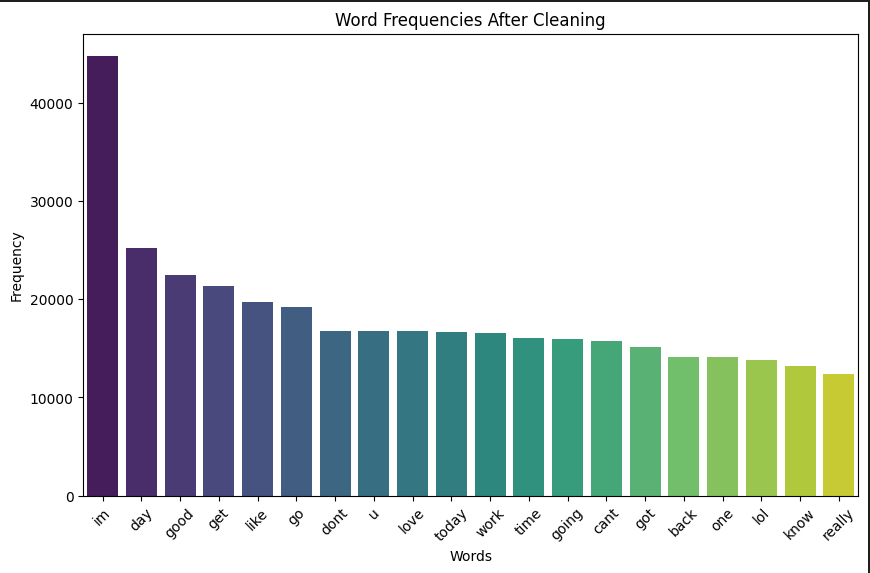
\includegraphics[width=\linewidth]{assets/Word_Freq_Chart.png}
        \caption{Word Frequency Chart}
        \label{fig:word_freq_chart}
    \end{figure}
      
\\
To further analyze sentiment, we created two word clouds: the first represented the most frequent words in positive tweets (Figure B),
 where the word "love" emerged as a dominant theme.
 \begin{figure}[H]
        \centering
        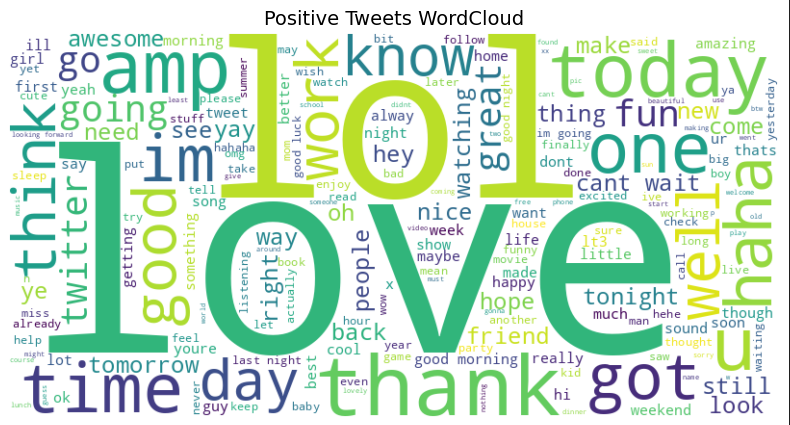
\includegraphics[width=\linewidth]{assets/PositiveWorldCloud.png}
        \caption{Word Frequency Chart}
        \label{fig:word_freq_chart}
    \end{figure} 
    \\
    The second word cloud depicted frequent words in negative tweets (Figure C), where the word "today" stood out. 
 These visualizations provided useful insights into the linguistic patterns present in positive and negative sentiments.
 \begin{figure}[H]
        \centering
        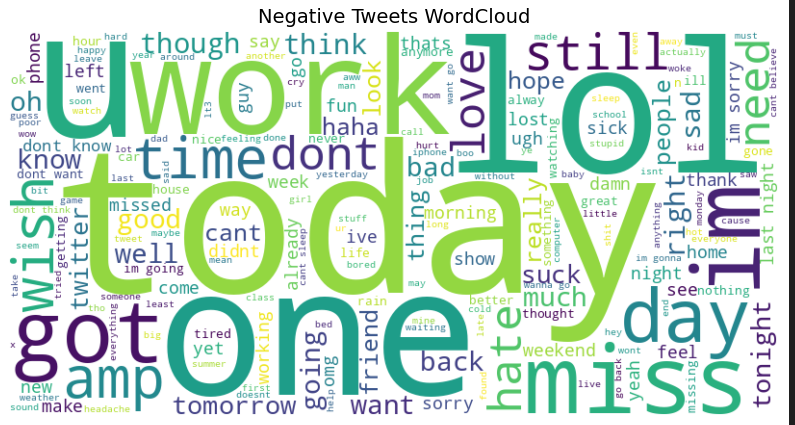
\includegraphics[width=\linewidth]{assets/NegativeWordCloud.png}
        \caption{Word Frequency Chart}
        \label{fig:word_freq_chart}
    \end{figure}
 \\
\section{Results and Evaluation}
The performance of the models was evaluated based on standard metrics used in classification tasks: accuracy, precision, recall, and F1-score. 
The results are as follows:

    Logistic Regression:
\\
        Accuracy: 85%
\\
        Precision: 84%
\\
        Recall: 83%
\\
        F1-score: 83%
\\
    Support Vector Machine (SVM):
\\
        Accuracy: 88%
\\
        Precision: 87%
\\
        Recall: 86%
\\
        F1-score: 86%
\\
The SVM model outperformed Logistic Regression in all evaluation metrics, achieving the highest accuracy and better precision and recall scores. 
A confusion matrix was also used to analyze the misclassifications, providing insights into how well the models differentiated between positive
 and negative tweets.
\section{conclusion}
This project demonstrated the application of machine learning models to classify sentiment in Twitter tweets. The SVM model proved to be the 
most effective in classifying the sentiment, providing better accuracy and recall than Logistic Regression. The key preprocessing steps—such as 
lemmatization, URL removal, and emoji handling—were crucial in improving the models' performance. Despite these improvements, challenges remain, 
particularly in detecting sarcasm and understanding the context of tweets, which are crucial for improving sentiment analysis. Future work could 
explore the use of deep learning models, such as BiLSTM, and tackle the problem of handling sarcasm and nuanced expressions in tweets. The findings
 have real-world applications in understanding public sentiment on social media platforms, with potential uses in business, politics, and social 
 research.
\section*{References}
Pang, B., Lee, L., & Vaithyanathan, S. (2002). Thumbs up? Sentiment classification using machine learning techniques. Proceedings of EMNLP, 79–86. 
\\
\\
Yoon Kim. 2014. Convolutional Neural Networks for Sentence Classification. In Proceedings of the 2014 Conference on Empirical Methods in Natural 
Language Processing (EMNLP), pages 1746–1751, Doha, Qatar. Association for Computational Linguistics
\begin{thebibliography}{00}
\bibitem
\end{thebibliography}
\vspace{12pt}

\end{document}
